\documentclass[tikz]{standalone}
\usepackage{pgfplots}
\pgfplotsset{compat=1.16}

\begin{document}
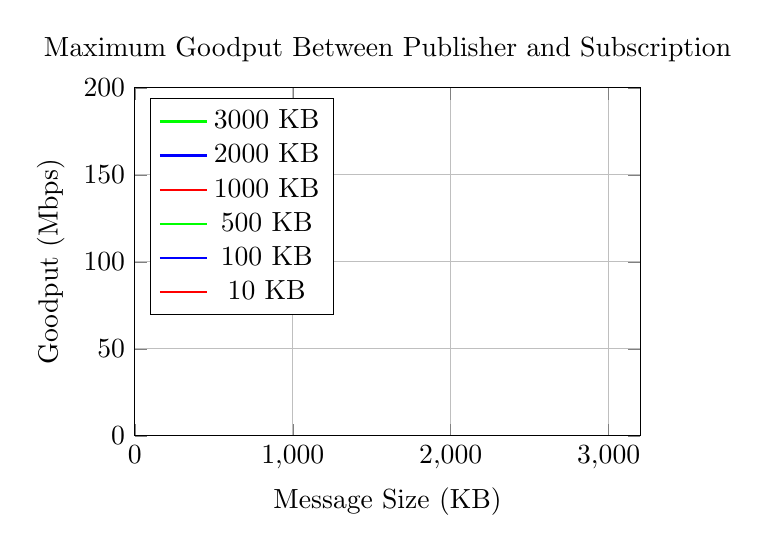
\begin{tikzpicture}
    \begin{axis}[
        title={Maximum Goodput Between Publisher and Subscription},
        xlabel={Message Size (KB)},
        ylabel={Goodput (Mbps)},
        xmin=0,
        xmax=3200,
        ymin=0,
        ymax=200,
        xtick={0, 1000, 2000, 3000},
        ytick={0, 50, 100, 150, 200},
        grid=major,
        legend pos=north west,
        width=8cm,
        height=6cm,
        ]
        
        % Define colors
        \definecolor{green}{RGB}{0, 255, 0}
        \definecolor{blue}{RGB}{0, 0, 255}
        \definecolor{red}{RGB}{255, 0, 0}
        
        % Plot data points
        \addplot[green, thick] coordinates {(3000, 180)};
        \addlegendentry{3000 KB}
        
        \addplot[blue, thick] coordinates {(2000, 140)};
        \addlegendentry{2000 KB}
        
        \addplot[red, thick] coordinates {(1000, 90)};
        \addlegendentry{1000 KB}
        
        \addplot[green, thick] coordinates {(500, 45)};
        \addlegendentry{500 KB}
        
        \addplot[blue, thick] coordinates {(100, 15)};
        \addlegendentry{100 KB}
        
        \addplot[red, thick] coordinates {(10, 5)};
        \addlegendentry{10 KB}
        
    \end{axis}
\end{tikzpicture}
\end{document}